% !TEX root = ../../Diploma.tex
\section{Learning a New Behaviour}
\subsection{Training with a long period and high discount factor}
Since it could be shown, that the agent can improve the static parameters of a control strategy, the next step is to attempt to train an agent to learn a new behaviour. As described in \ref{ssec:new_behaviour_description}, three agents controlling the generator torque of the three turbines are trained. First, an agent with a long update period and a high discount factor will be examined. The long update period is chosen to allow the agent to develop lower frequency strategies. As was noted in \autoref{ssec:new_behaviour_description}, a high discount factor is chosen from an analysis of the physical timescales of the wind park.
\begin{figure}[h]
	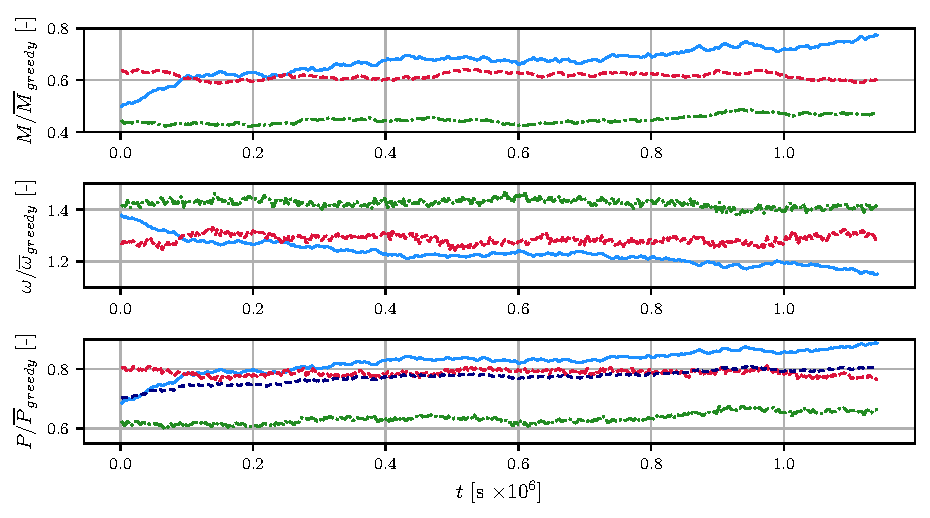
\includegraphics{plots/behaviour_optimization/torque_long_high_training.pdf}
	\caption{\legendFive{Turbine 0}{Turbine 1}{Turbine 2}{Total}{Greedy.} Training of agent with $\gamma=0.99$ and for periods with $N_{a,e}=1500$.}
	\label{fig:torque_long_high_training}
\end{figure}\\
The timeseries of the generator torques, the angular velocities and the generated power of the three turbines as well as the total generated power are shown in \autoref{fig:torque_long_high_training}. It shows that after $\SI{1.2e6}{s}$ the performance by the agent is still significantly worse than that of a greedy controller. Therefore the training was stopped at this point. Furthermore, no improvement in total power is visible for $\SI{1e5}{s}$. The figure shows, that the torque of the first turbine is steadily increased throughout the training, while the torque of the second and third turbine show little change.
\begin{figure}[h]
	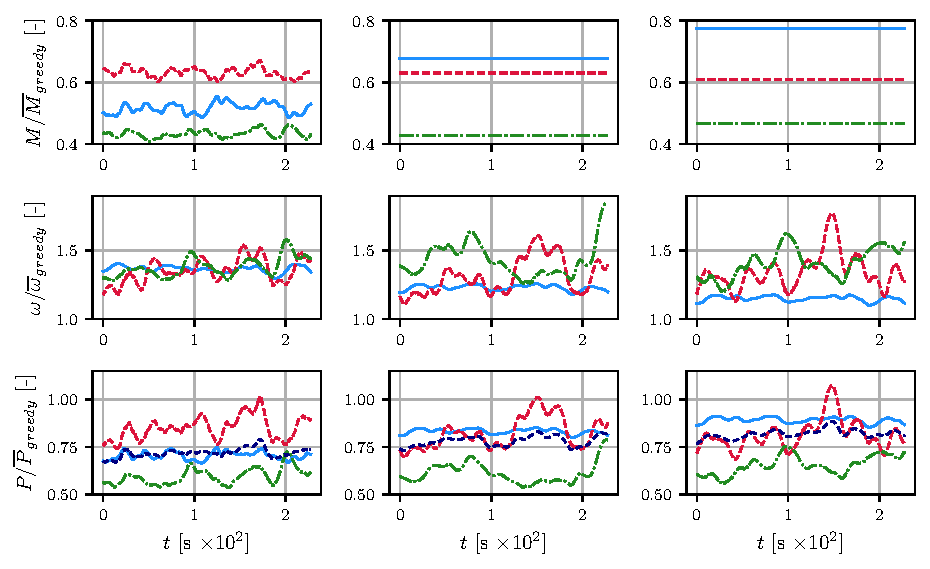
\includegraphics{plots/behaviour_optimization/torque_long_high_eval.pdf}
	\caption{\legendFive{Turbine 0}{Turbine 1}{Turbine 2}{Total}{Greedy.}Evolution of control strategy of agent with $\gamma=0.99$ and for periods with $N_{a,e}=1500$. Left column is control strategy in the beginning of training, central column after half of the training and right column after training has finished.}
	\label{fig:torque_long_high_eval}
\end{figure} \\
To analyze the evolution of the control strategy, despite it not being successful, \autoref{fig:torque_long_high_eval} shows generator torque, angular velocity and generated power by the turbines when controlled by the agent after 12 updates, after half of training time and after the full training time. The comparison of the control strategies shows that the agent evolves to set a constant generator torque at all three turbines. This is already visible after half of the training time. Furthermore, as was seen in \autoref{fig:torque_long_high_training}, the generator torque of the first turbine increases, while the torque at the other two turbines does not change after half of the training. Since the power of the first turbine is greatest, it appears reasonable that control of that turbine is improved fastest. A static generator torque differs from greedy control, but considering that the inflow has a uniform mean value, such a strategy still can be reasonable. However, since the total generated power only reached about three quarter of the total power of a greedy-controlled park, this strategy will not be investigated further. The major drawback of this agent was the slow evolution. One of the possible reasons for this is the long period between updates. Furthermore, the reason for the long period was the ability to develop lower frequency behaviour, which did not occur. Therefore another agent with a shorter update period was trained.
\subsection{Training with a short period and high discount factor}
To increase the number of updates per simulated time, an agent with a number of actions per episode of 500 was trained.  
\begin{figure}[h]
	\centering
	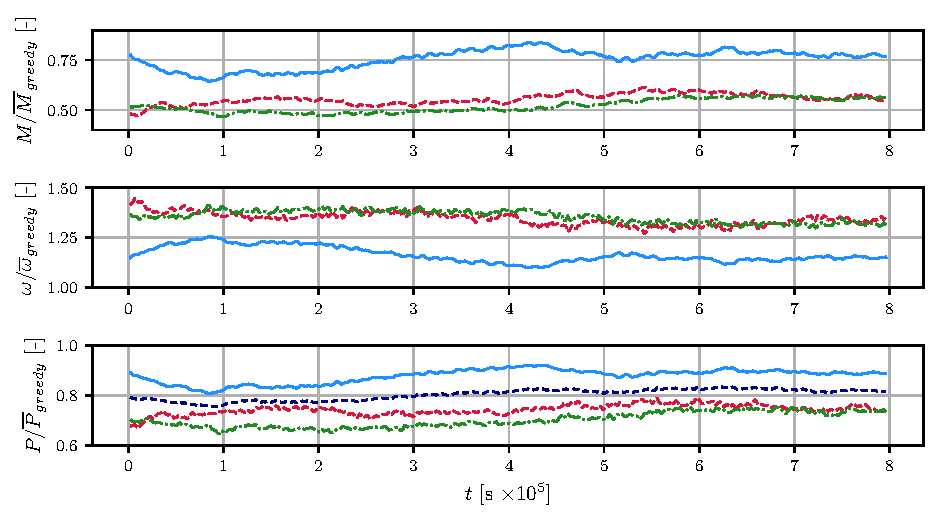
\includegraphics{plots/behaviour_optimization/torque_short_high_training.pdf}
	\caption{\legendFive{Turbine 0}{Turbine 1}{Turbine 2}{Total}{Greedy.}Training of agent with $\gamma=0.99$ and for periods with $N_{a,e}=500$.}
	\label{fig:torque_short_high_training}
\end{figure}\\
The time series of the generated power, angular velocity and generator torque are shown in \autoref{fig:torque_short_high_training}. It shows that total generated power, after an initial decrease, increased for about half of the training. After that, total power did not increase, but the mean of the controlled variables, the generator torques, still changed. Therefore training was continued further, but the agent returned to the same state multiple times. Thus training was stopped after $\SI{8e5}{s}$. The comparison to the previous agent with a longer period shows, that the behaviour of the agent changes faster. Yet it is not able to develop a strategy that performs as good as a greedy controller. While the first turbine performs almost as good as a single greedy controlled turbine, the second and the third turbine perform considerably worse. The plot also shows that little changes occur in the control strategy for these two turbines. Again, this can be explained by the larger power produced at the first turbine. 
\begin{figure}[h]
	\centering
	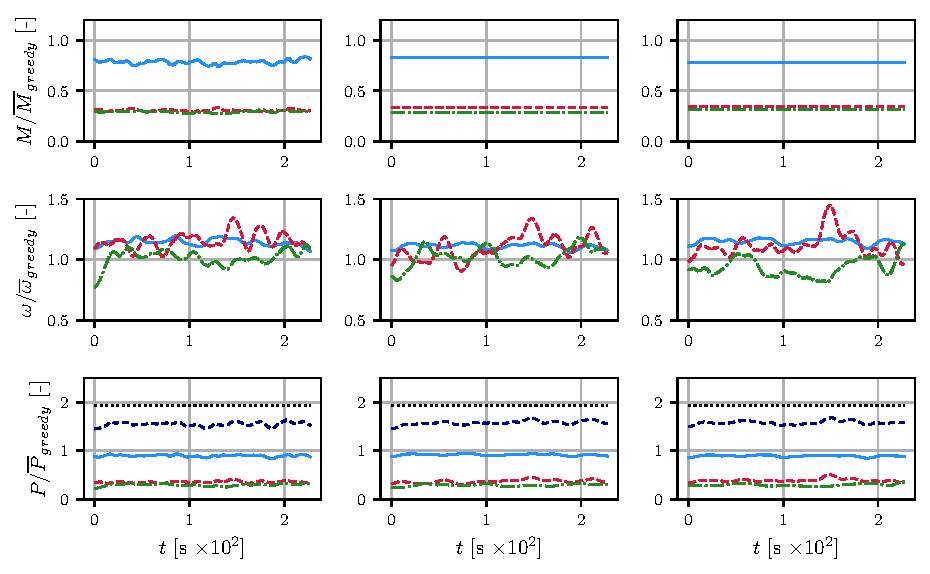
\includegraphics{plots/behaviour_optimization/torque_short_high_eval.pdf}
	\caption{\legendFive{Turbine 0}{Turbine 1}{Turbine 2}{Total}{Greedy.}Evolution of control strategy of agent with $\gamma=0.99$ and for periods with $N_{a,e}=500$. Left column is control strategy in the beginning of training, central column after half of the training and right column after training has finished.}
	\label{fig:torque_short_high_eval}
\end{figure}
To find out more about the developed strategy and how it changed throughout the training, \autoref{fig:torque_short_high_eval} shows generator torques, angular velocities and generated powers per turbine as well as total generated power for parks controlled by agents at the beginning of the training, after half the training and after training has been completed. It shows that this agent also developed the strategy to set constant generator torques.  It also  shows that the first turbine performs almost as good as a greedy controlled turbine. In comparison to the greedy controller the agent sets a lower generator torque at all of the turbines, therefore they have higher angular velocities. Thus the thrust forces exerted by the turbines are also higher, resulting in a higher wake deficit. Consequentially the downstream turbines perform worse. However it is not clear why the agent does not set higher torques to reduce thrust. As was explained in \autoref{ssec:new_behaviour_description}, the high discount rate leads to consideration of rewards that occur far in the future. This leads to a noisy signal, where influences of later actions also play a role. In combination with a turbulent flow that is by definition noisy, this might inhibit optimization as no strong correlation between return, which is the discounted sum of total generated power, and generator torque at one point in time exists. To reduce the noise in the signal an agent is trained with a lower discount rate.
\subsection{Training with a short period and low discount factor}
While a discount rate of $\gamma=0.99$ allows for the return to include the influence the action at the first turbine has with power produced by the second turbine after that information has been carried there, it might also lead to incorporation of too many timesteps into the return, thus making it impossible for the agent to improve its behaviour. Therefore an agent with a discount rate of $\gamma=0.95$ was trained as well.
\begin{figure}[h]
	\centering
	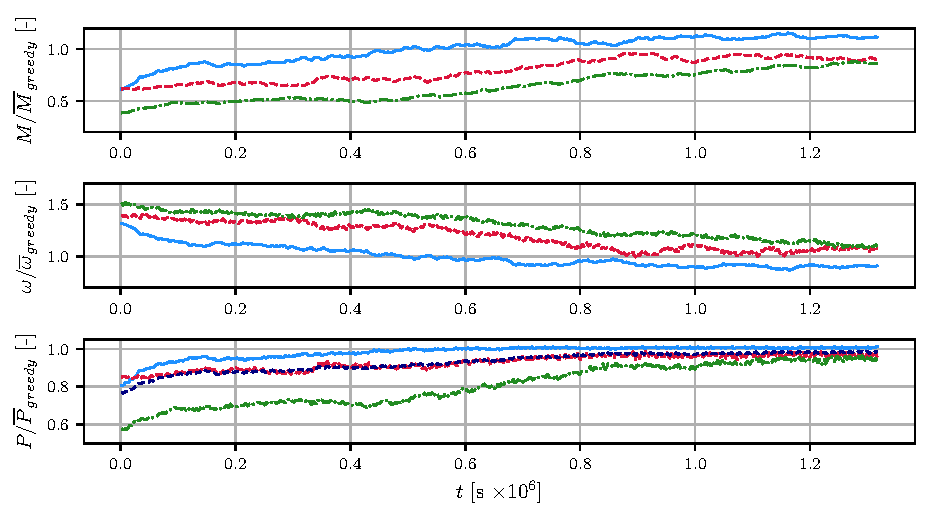
\includegraphics{plots/behaviour_optimization/torque_short_low_training.pdf}
	\caption{\legendFive{Turbine 0}{Turbine 1}{Turbine 2}{Total}{Greedy.}Training of agent with $\gamma=0.95$ and for periods with $N_{a,e}=500$.}
	\label{fig:torque_short_low_training}
\end{figure} \\
The time series of the training of that agent is shown in \autoref{fig:torque_short_low_training}. This agent did learn a behaviour that performs almost as good as the greedy control. While the gain in total power in the beginning of training can be attributed to an increase in power produced by the first turbine, the third turbine also improves continuously. The second turbine also improves in power with time, although the gains are smaller. The training is conducted for $\SI{1.3e6}{s}$, which is longer than for the previous agents, but the strategy had not finished improving after $\SI{8e5}{s}$. A look at the generator torques shows that the torque at all three turbines increased throughout the training, which in turn lead to a decrease in angular velocity at all three turbines. The overall development of power and torque looks similar to that of the first agent as shown in \autoref{fig:torque_long_high_training}. As length of training period and discount factor both influence the return, both these agents seem to have a good ratio of these factors. As the long period agent did not develop a dynamic control strategy, the long period does not offer advantages, but only increases the simulated time per update. 
\begin{figure}[h]
	\centering
	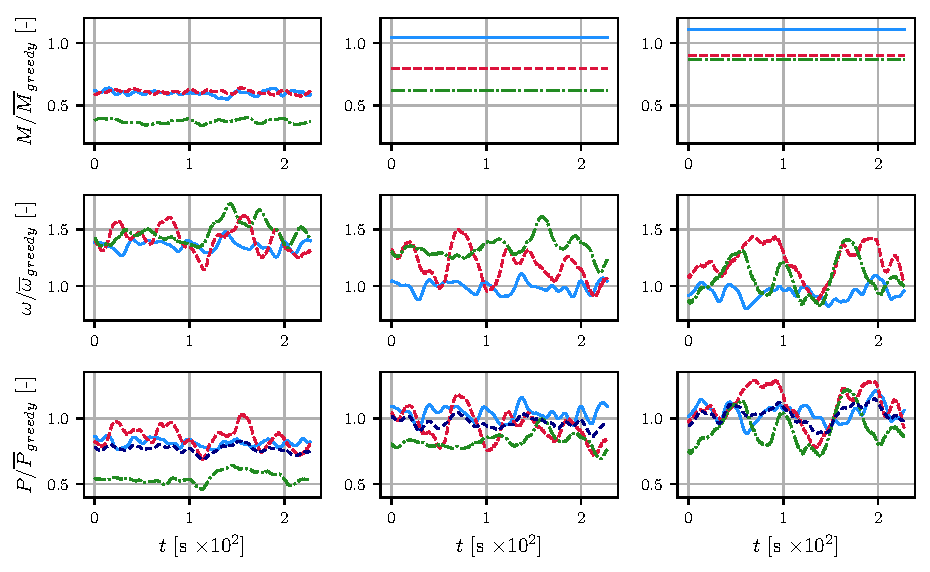
\includegraphics{plots/behaviour_optimization/torque_short_low_eval.pdf}
	\caption{\legendFive{Turbine 0}{Turbine 1}{Turbine 2}{Total}{Greedy.}Evolution of control strategy of agent with $\gamma=0.95$ and for periods with $N_{a,e}=500$. Left column is control strategy in the beginning of training, central column after half of the training and right column after training has finished.}
	\label{fig:torque_short_low_eval}
\end{figure} \\
The evolution of the strategy is shown in \autoref{fig:torque_short_low_eval}. It shows that this agent, like the other two previously studied, sets a constant generator torque after half of the training and does not react to the flow any more. The strategy in the second half of the training only changes in the constant torque that is set. As was visible in \autoref{fig:torque_short_low_training}, the torques set all increase in value. The final control strategy sets a higher torque at the first turbine than the mean torque set by a greedy controller. Furthermore it shows that, since a constant generator torque is set, angular velocities fluctuate due to the turbulent inflow. Furthermore these fluctuations are also visible in the generated power. As was mentioned in the analysis of the first generator torque controlling agent, one reason for the development of the static strategy might be that the mean inflow velocity is constant and only superimposed with fluctuations. Thus in the mean this strategy is comparable to a very slow greedy controller.
\subsection{Analysis of flow}
\begin{table}[h]
	\centering
	\caption{Mean, relative difference in mean and relative in standard deviation of power and aerodynamic moment of a trained torque-controlling agent in comparison to the greedy-control case.}
	\begin{tabular}{ccccccc}
		\toprule
		& \multicolumn{3}{c}{$P$}  & \multicolumn{3}{c}{$M_{aero}$ }\\ \cmidrule(rl){2-4} \cmidrule(rl){5-7}
		& mean & rel. mean & rel. std  & mean & rel. mean & rel. std \\ \midrule
		Total & $\SI{  9.65}{MW} $ & $\SI{ -1.42}{\%}$ & $\SI{ -19.3}{\%}$ &-&-&- \
		\\
		Turbine 0  & $\SI{   5.1}{MW} $ & $\SI{+0.837}{\%}$ & $\SI{ +6.28}{\%}$ & $\SI{3.53e03}{kNm} $ & $\SI{ +10.6}{\%}$ & $\SI{ +14.8}{\%}$ \\
		Turbine 1  & $\SI{  2.48}{MW} $ & $\SI{ -3.23}{\%}$ & $\SI{ -22.5}{\%}$ & $\SI{1.82e03}{kNm} $ & $\SI{ -9.65}{\%}$ & $\SI{ -4.19}{\%}$ \\
		Turbine 2  & $\SI{  2.07}{MW} $ & $\SI{ -4.55}{\%}$ & $\SI{ -26.1}{\%}$ & $\SI{1.57e03}{kNm} $ & $\SI{ -13.2}{\%}$ & $\SI{ -6.25}{\%}$ \\
		\bottomrule
	\end{tabular}
	\label{tab:torque_quants}
\end{table}
In \autoref{tab:torque_quants} mean values as well as relative changes in mean and standard deviation compared to a greedy controlled case are shown for power and aerodynamic torque. The total power production is $1.42$ percent lower than that of a greedy controlled park. This is due to decreases in power produced by the second and third turbine, while first turbine produces negligibly more. But while the primary objective, the increase in total power could not be reached, the quality of overall power significantly improved with a reduction in standard deviation of $19.3$ percent. This is due to a decrease in fluctuations at the second and third turbine, while fluctuations at the first turbine increased. The same is true for the aerodynamic moment. The mean as well as the standard deviation increased at the first turbine while they were considerably reduced at the second and third turbine. As especially power quality is of growing concern, a more thorough analysis of the flow might offer insights into how this reduction is achieved.
\begin{figure}[h]
	\centering
	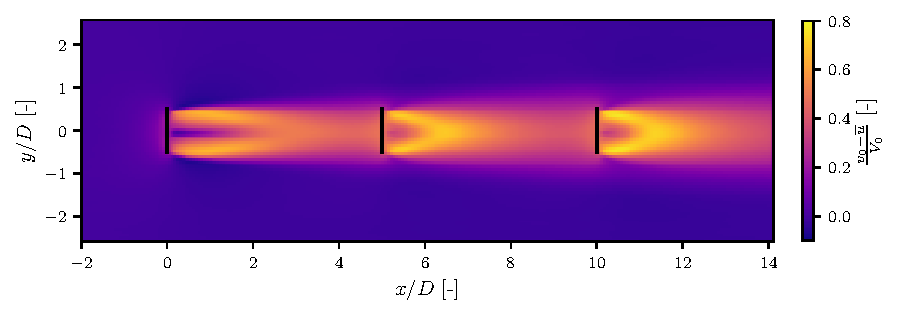
\includegraphics{plots/behaviour_optimization/torque_short_low_velocity.pdf}
	\caption{{\color{black} \rule[3pt]{22pt}{1pt} Turbine.} Mean .}
	\label{fig:torque_vel}
\end{figure} \\
To this end, \autoref{fig:torque_vel} shows the velocity wake deficit in the domain. 
\begin{figure}[h]
	\centering
	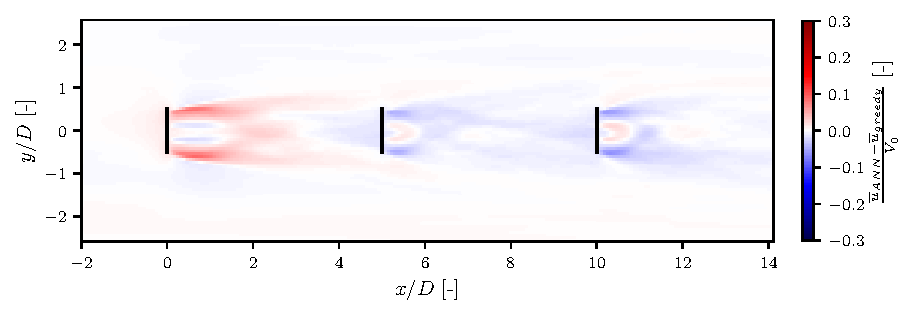
\includegraphics{plots/behaviour_optimization/torque_short_low_velocity_difference.pdf}
	\caption{{\color{black} \rule[3pt]{22pt}{1pt} Turbine.} Turbulence intensity of optimized helix control.}
\end{figure}
\begin{figure}[h]
	\centering
	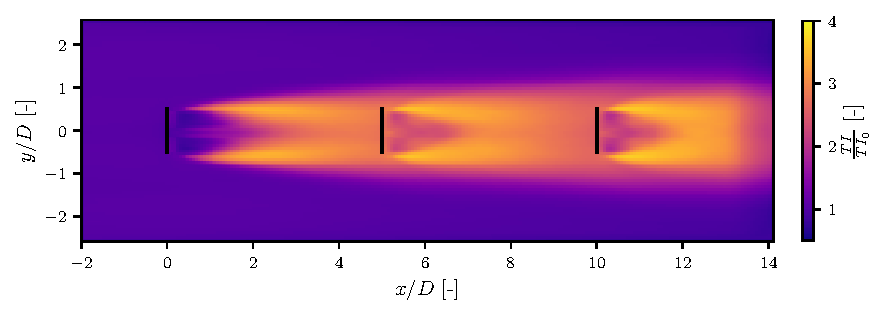
\includegraphics{plots/behaviour_optimization/torque_short_low_turbulence_intensity.pdf}
	\caption{{\color{black} \rule[3pt]{22pt}{1pt} Turbine.} Turbulence intensity of optimized helix control.}
\end{figure}
\begin{figure}[h]
	\centering
	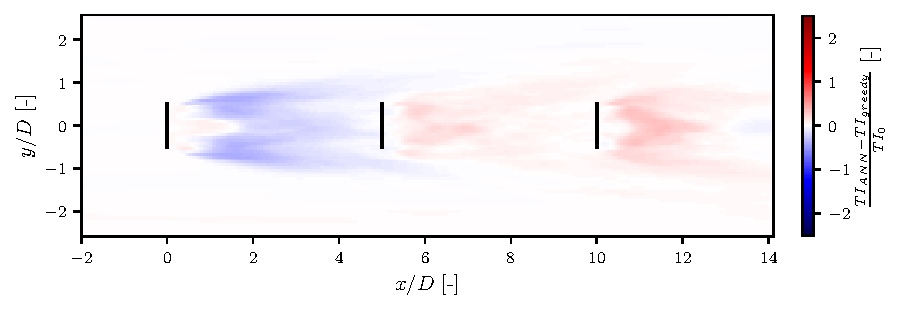
\includegraphics{plots/behaviour_optimization/torque_short_low_ti_difference.pdf}
	\caption{{\color{black} \rule[3pt]{22pt}{1pt} Turbine.} Turbulence intensity of optimized helix control.}
\end{figure}

